% % -*- coding:utf-8 -*-
\documentclass[aspectratio=169,10pt]{beamer}
\nonstopmode

\usepackage{appendixnumberbeamer}
\usepackage{graphicx}
\usepackage{url}
\usepackage{amsmath, amssymb}
\usepackage{pifont} %fuer checkmarks
% color palette
\definecolor{tu01}{HTML}{84B818}
\definecolor{tu02}{HTML}{D18B12}
\definecolor{tu03}{HTML}{1BB5B5}
\definecolor{tu04}{HTML}{F85A3E}
\definecolor{tu05}{HTML}{4B6CFC}
\definecolor{tu06}{HTML}{E3B505}
\definecolor{tu07}{HTML}{AF331D}
\definecolor{tu08}{HTML}{000000}
\definecolor{tu09}{HTML}{AAAAAA}
\definecolor{tu10}{HTML}{444444}
\definecolor{tu11}{HTML}{84B818}

% mixed and light colors
\colorlet{tu01light}{tu01!33}
\colorlet{tu02light}{tu02!33}
\colorlet{tu03light}{tu03!33}
\colorlet{tu04light}{tu04!33}
\colorlet{tu05light}{tu05!33}
\colorlet{tu06light}{tu06!33}
\colorlet{tu07light}{tu07!33}
\colorlet{tu08light}{tu08!33}
\colorlet{tu09light}{tu09!33}
\colorlet{tu10light}{tu10!33}
\colorlet{tu11light}{tu11!33}

\colorlet{tu01midlight}{tu01!50}
\colorlet{tu02midlight}{tu02!50}
\colorlet{tu03midlight}{tu03!50}
\colorlet{tu04midlight}{tu04!50}
\colorlet{tu05midlight}{tu05!50}
\colorlet{tu06midlight}{tu06!50}
\colorlet{tu07midlight}{tu07!50}
\colorlet{tu08midlight}{tu08!50}
\colorlet{tu09midlight}{tu09!50}
\colorlet{tu10midlight}{tu10!50}
\colorlet{tu11midlight}{tu11!50}

\colorlet{tu01dark}{tu01!80!black}
\colorlet{tu02dark}{tu02!80!black}
\colorlet{tu03dark}{tu03!80!black}
\colorlet{tu04dark}{tu04!80!black}
\colorlet{tu05dark}{tu05!80!black}
\colorlet{tu06dark}{tu06!80!black}
\colorlet{tu07dark}{tu07!80!black}
\colorlet{tu08dark}{tu08!80!black}
\colorlet{tu09dark}{tu09!80!black}
\colorlet{tu10dark}{tu10!80!black}
\colorlet{tu11dark}{tu11!80!black}

\colorlet{lightgray}{gray!25}
\colorlet{midlightgray}{gray!50}
\colorlet{anthracite}{black!85}

% aliases
\colorlet{tudo}{tu01}
\colorlet{tuorange}{tu02}
\colorlet{tudolight}{tu01light}

% \usepackage{beamerthememetropolis}
\usetheme[progressbar=frametitle,noslidenumbers]{metropolis}
\newcommand{\themename}{\textbf{\textsc{metropolis}}\xspace}


\usepackage{xcolor}


\title{Abschlusspr\"asentation Projekt 2}
% \subtitle{Learning to Identify Similarities between Mathematical Expressions}
\author{Pouria Araghchi 170468, Kai Lukas Ilmenau 225338, Naveed Niazi 214471}

\institute{TU Dortmund - Fachprojekt zu "Routingalgorithmen"}
\titlegraphic{\hfill
\includegraphics[height=8mm]{tu-do-logo.pdf}}

\date{\today}

\begin{document}

\maketitle
% %%%%%%%%%%%%%%%%%%%%%%%%%%%%%%%%%%%%%%%%%%%%%%%%%%%
% %%%%%%%%%%%%%%%%%%%%%%%%%%%%%%%%%%%%%%%%%%%%%%%%%%%
% Kai
% %%%%%%%%%%%%%%%%%%%%%%%%%%%%%%%%%%%%%%%%%%%%%%%%%%%
% %%%%%%%%%%%%%%%%%%%%%%%%%%%%%%%%%%%%%%%%%%%%%%%%%%%
\section{Kai}

\begin{frame}{Die Topologie}
\begin{columns}
\begin{column}[t]{0.7\paperwidth}
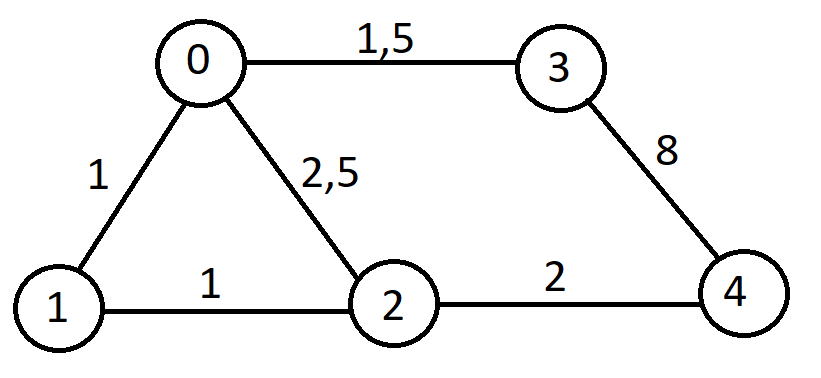
\includegraphics[width=\textwidth]{images/kai1.png}
\end{column}
\begin{column}[t]{0.3\paperwidth}
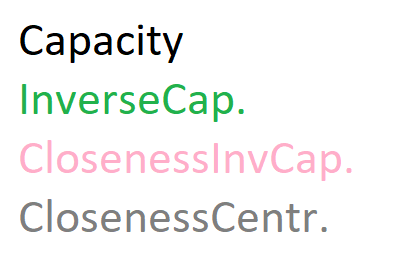
\includegraphics[width=\textwidth]{images/kai_legend.png}
\end{column}
\end{columns}
\end{frame}

\begin{frame}{Inverse Capacity}
\begin{columns}
\begin{column}[t]{0.7\paperwidth}
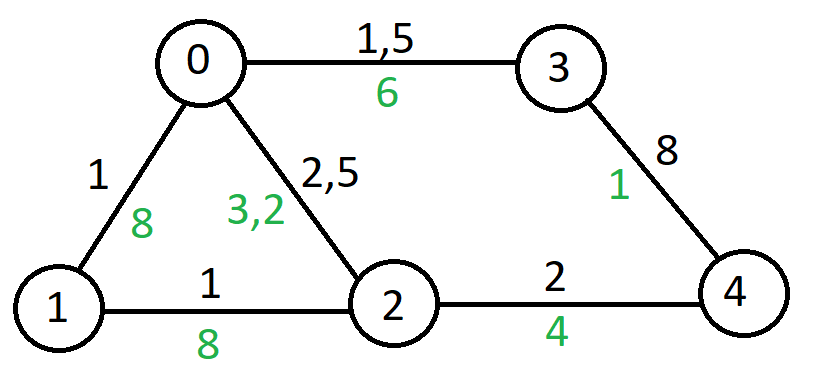
\includegraphics[width=\textwidth]{images/kai2.png}
\end{column}
\begin{column}[t]{0.3\paperwidth}
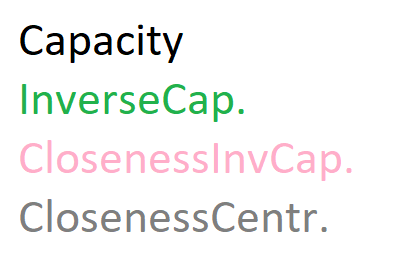
\includegraphics[width=\textwidth]{images/kai_legend.png}
\end{column}
\end{columns}
\end{frame}

\begin{frame}{Closeness Centrality Werte}
\begin{columns}
\begin{column}[t]{0.7\paperwidth}
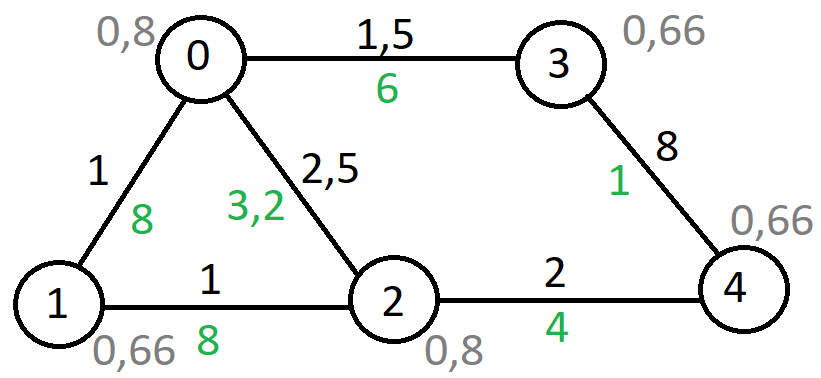
\includegraphics[width=\textwidth]{images/kai3.png}
\end{column}
\begin{column}[t]{0.3\paperwidth}
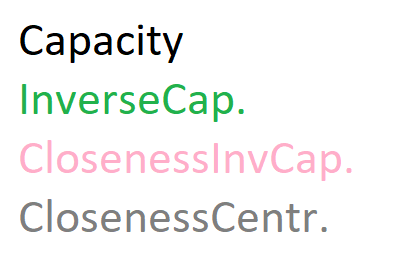
\includegraphics[width=\textwidth]{images/kai_legend.png}
\end{column}
\end{columns}
\end{frame}

\begin{frame}{Closeness Centrality With Inverse Capacity}
\begin{columns}
\begin{column}[t]{0.7\paperwidth}
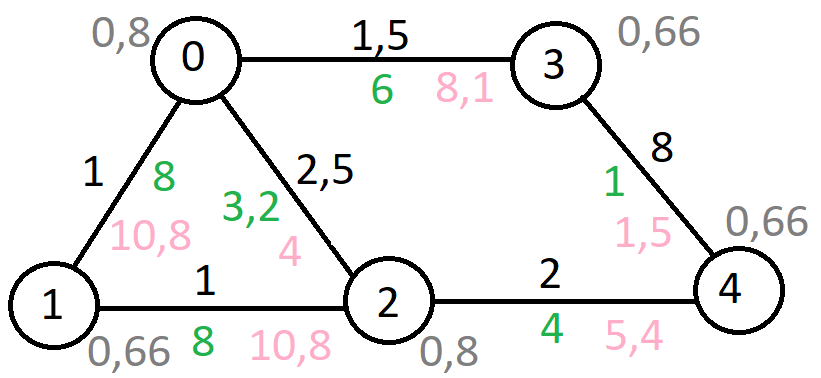
\includegraphics[width=\textwidth]{images/kai4.png}
\end{column}
\begin{column}[t]{0.3\paperwidth}
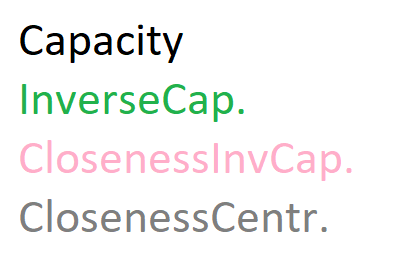
\includegraphics[width=\textwidth]{images/kai_legend.png}
\end{column}
\end{columns}
\end{frame}

\begin{frame}{Mit Demands}
\begin{columns}
\begin{column}[t]{0.7\paperwidth}
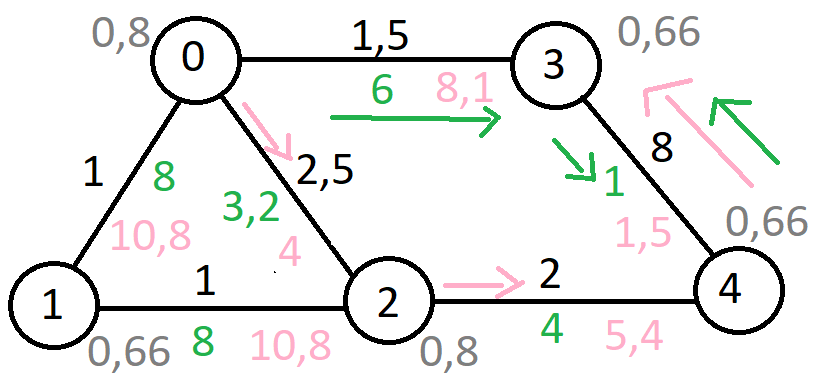
\includegraphics[width=\textwidth]{images/kai5.png}
\Large
Demands von 0 nach 4 (eine Capacity-Einheit) und von 4 nach 3 (acht Capacity-Einheiten)
\end{column}
\begin{column}[t]{0.3\paperwidth}
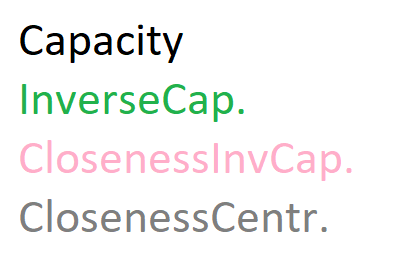
\includegraphics[width=\textwidth]{images/kai_legend.png}
\end{column}
\end{columns}
\end{frame}

\begin{frame}{Boxplots}
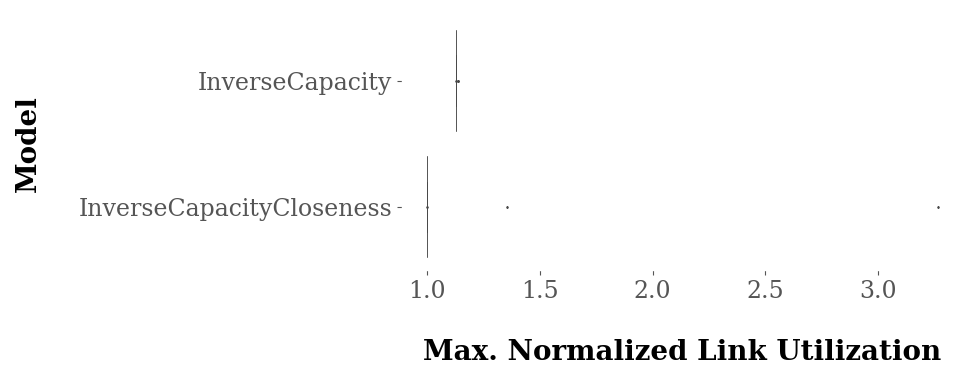
\includegraphics[width=\textwidth]{images/kai6.png}
\end{frame}

\begin{frame}{Ist meine Algorithmus besser?}
\Large
\begin{itemize}
    \item in diesem speziellen Setting: Ja
    \item "designed" Topologie\newline
    $\rightarrow$ lange Suche nach guter Topologie f\"ur den Algorithmus
    \item Siehe Projekt 1: $Inverse\_Capacity$ im Durchschnitt besser als meine Anpassung
\end{itemize}
\end{frame}
% %%%%%%%%%%%%%%%%%%%%%%%%%%%%%%%%%%%%%%%%%%%%%%%%%%%
% %%%%%%%%%%%%%%%%%%%%%%%%%%%%%%%%%%%%%%%%%%%%%%%%%%%
% Naveed
% %%%%%%%%%%%%%%%%%%%%%%%%%%%%%%%%%%%%%%%%%%%%%%%%%%%
% %%%%%%%%%%%%%%%%%%%%%%%%%%%%%%%%%%%%%%%%%%%%%%%%%%%
\section{Naveed}
\begin{frame}[fragile]{}
\begin{center}
    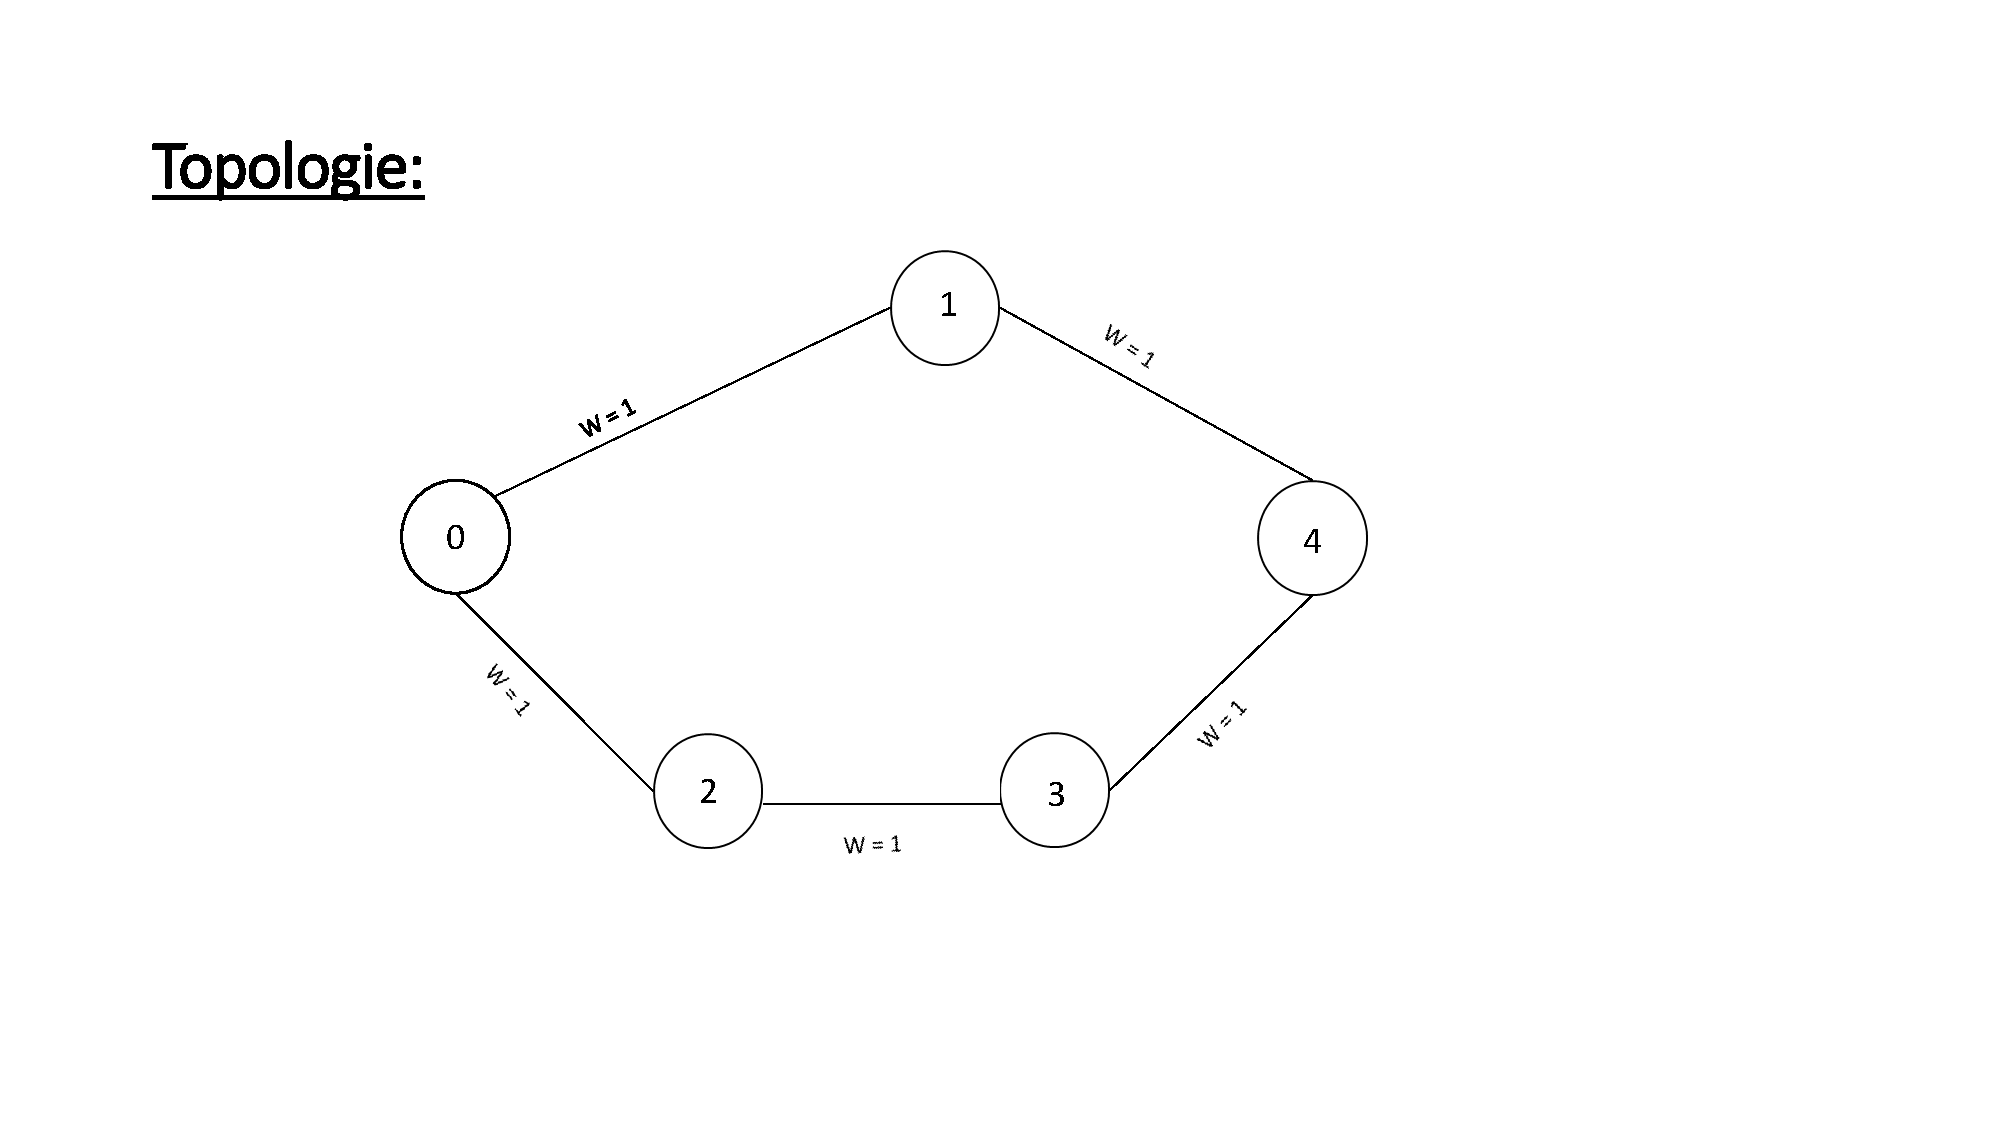
\includegraphics[width=\textwidth]{images/naveed_1.pdf}
\end{center}
\end{frame}
\begin{frame}{Ergebnisse}
\begin{center}
    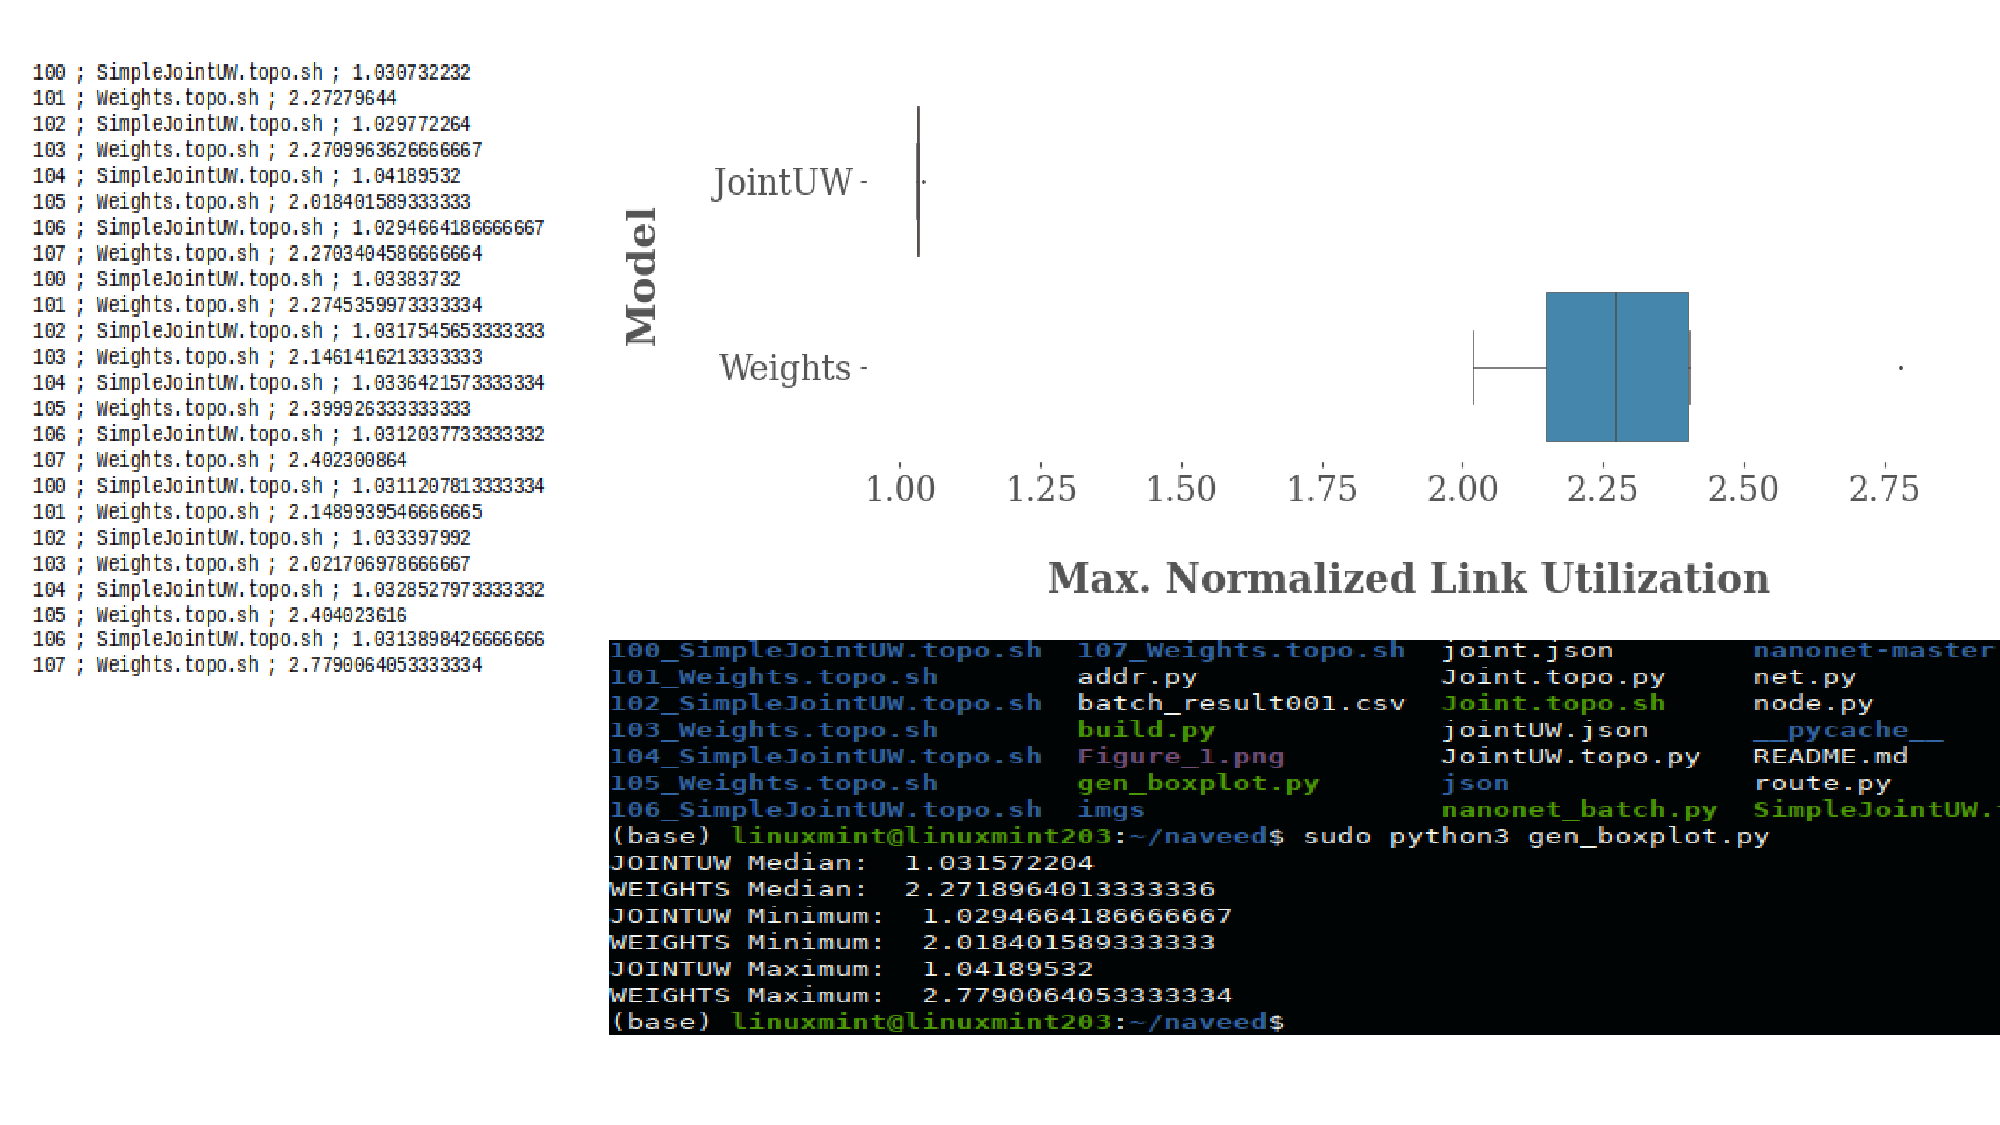
\includegraphics[width=\textwidth]{images/naveed_2.pdf}
\end{center}
\end{frame}

% %%%%%%%%%%%%%%%%%%%%%%%%%%%%%%%%%%%%%%%%%%%%%%%%
% Pouria
% %%%%%%%%%%%%%%%%%%%%%%%%%%%%%%%%%%%%%%%%%%%%%%%%

% %%%%%%%%%%%%%%%%%%%%%%%%%%%%%%%%%%%%%%%%%%%%%%%%%%%
% %%%%%%%%%%%%%%%%%%%%%%%%%%%%%%%%%%%%%%%%%%%%%%%%%%%
% Pouria
% %%%%%%%%%%%%%%%%%%%%%%%%%%%%%%%%%%%%%%%%%%%%%%%%%%%
% %%%%%%%%%%%%%%%%%%%%%%%%%%%%%%%%%%%%%%%%%%%%%%%%%%%
\section{Sequential Combination aus InverseCapacity und DemandFirstWaypoints}
% %%%%%%%%%%%%%%%%%%%%%%%%%%%%%%%%%%%%%%%%%%%%%%%%
% erste Folie
\begin{frame}{Netzwerktopologie (Anlehnung an Abilene)\footnote{FaPro\_P2/pouria/network\_origin.pdf}}
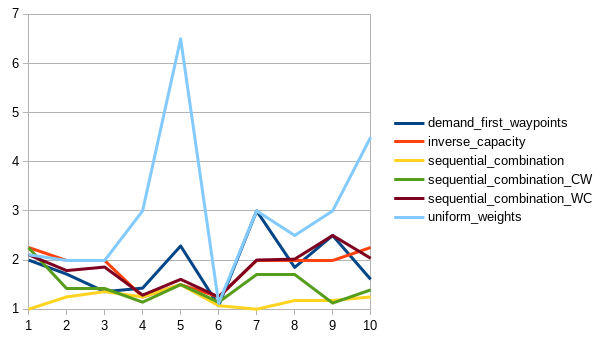
\includegraphics[width=\textwidth]{images/pouria1.png}
\end{frame}
% %%%%%%%%%%%%%%%%%%%%%%%%%%%%%%%%%%%%%%%%%%%%%%%%
% zweite Folie
\begin{frame}{Anwendung von InverseCapacity\footnote{FaPro\_P2/pouria/network\_origin.pdf}}
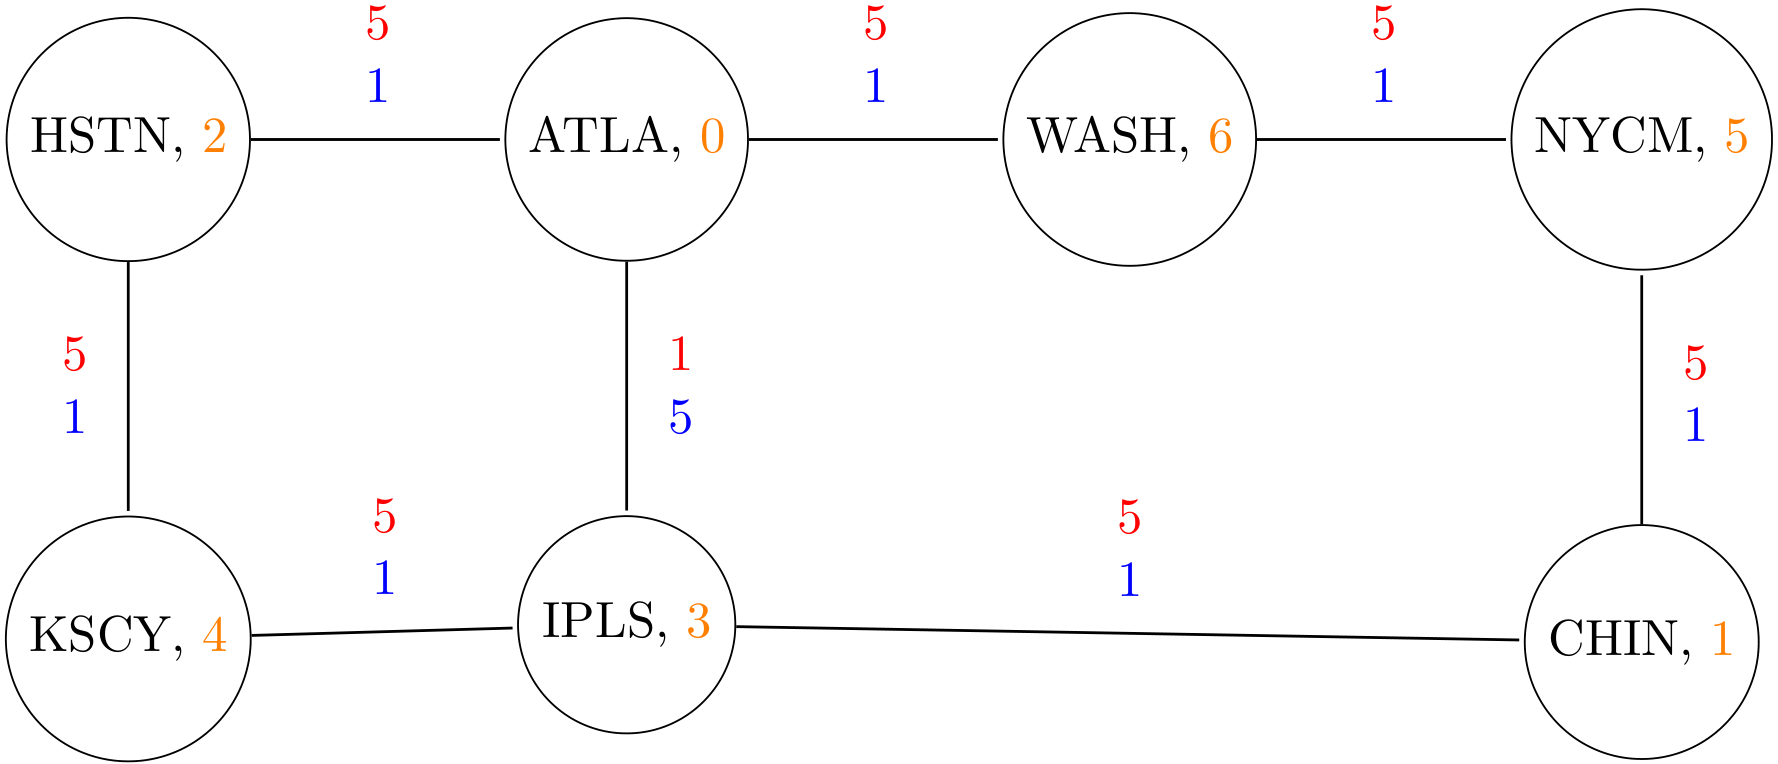
\includegraphics[width=\textwidth]{images/pouria2.png}
\end{frame}
% %%%%%%%%%%%%%%%%%%%%%%%%%%%%%%%%%%%%%%%%%%%%%%%%
% dritte Folie
\begin{frame}{Demandtabelle (vereinfacht)\footnote{FaPro\_P2/pouria/network\_origin.pdf}}
\centering
\begin{tabular}{c|c|c|c|c|c|c|c}
$\downarrow$ von, nach $\rightarrow$ & HSTN  & KSCY & ATLA   & IPLS  & CHIN  & WASH  & NYCM\\
\hline
HSTN    & & 1 & 13 & 2 & 6 & 8 & 3\\
\hline
KSCY    & 1 & & 1 & 2 & 4 & 2 & 2\\
\hline
ATLA    & 28 & 1 & & 5 & 3 & 19 & 4\\
\hline
IPLS    & 7 & 2 & 4 & & 14 & 7 & 9\\
\hline
CHIN    & 165 & 17& 18 & 7 & & 11 & 12\\
\hline
WASH    & 13 & 5 & 13  & 5 & 17 & &20\\
\hline
NYCM    & 16 & 3 & 9 & 4 & 61 & 24 & 
\end{tabular}
\end{frame}
% %%%%%%%%%%%%%%%%%%%%%%%%%%%%%%%%%%%%%%%%%%%%%%%%
% vierte Folie
\begin{frame}{Demandtabelle (st\"arker vereinfacht)\footnote{FaPro\_P2/pouria/network\_origin.pdf}}
\centering
\begin{tabular}{c|c|c|c|c|c|c|c}
$\downarrow$ von, nach $\rightarrow$ & HSTN  & KSCY & ATLA   & IPLS  & CHIN  & WASH  & NYCM\\
\hline
HSTN    & & & & & & & \\
\hline
KSCY    & & & & & & & \\
\hline
ATLA    & & & & 5 & & & \\
\hline
IPLS    & & & & & & 7 & \\
\hline
CHIN    & & & & & & & \\
\hline
WASH    & & & & & & & \\
\hline
NYCM    & & & & & & & 
\end{tabular}
\end{frame}
% %%%%%%%%%%%%%%%%%%%%%%%%%%%%%%%%%%%%%%%%%%%%%%%%
% neue Folien
\begin{frame}{Resultierender Boxplot}
\begin{columns}
\begin{column}[t]{0.5\paperwidth}
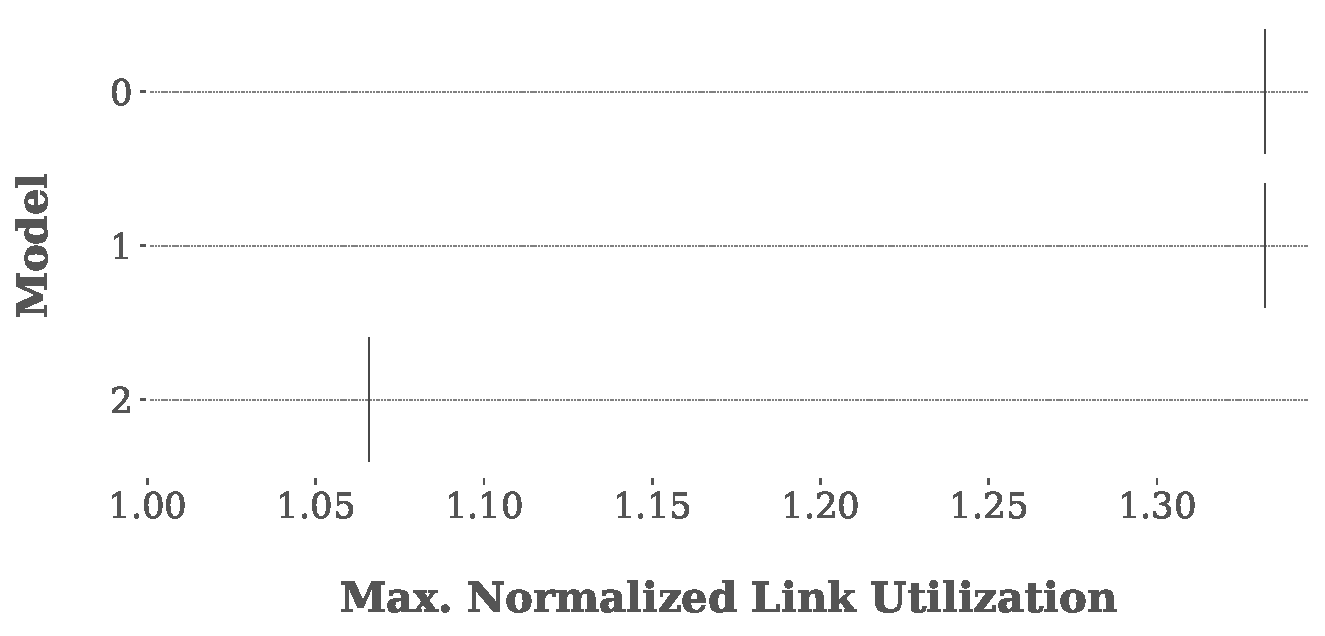
\includegraphics[width=\textwidth]{images/pouria3.pdf}
\end{column}
\begin{column}[t]{0.5\paperwidth}
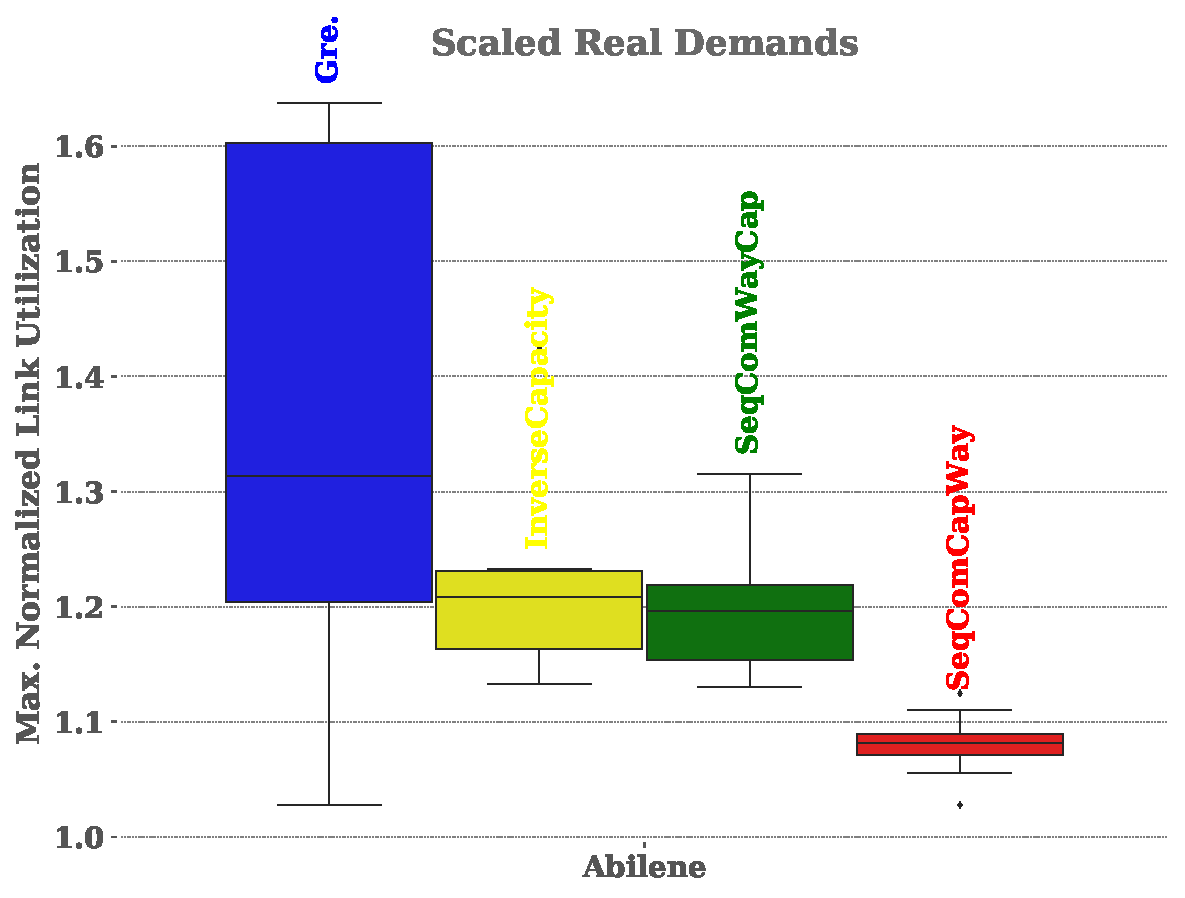
\includegraphics[width=\textwidth]{images/pouria_real_demands.pdf}
\end{column}
\end{columns}
\end{frame}
% %%%%%%%%%%%%%%%%%%%%%%%%%%%%%%%%%%%%%%%%%%%%%%%%
% neue Folien
\begin{frame}{Probleme}
\Large
\begin{itemize}
    \item keine Boxen:\newline
    $\rightarrow$ vermutlich zu schwacher Rechner (2 Minuten Timeout reicht nicht)
    \item Sequential Combination besser:\newline
    $\rightarrow$ meine Topolgie wurde vereinfacht, von Grund auf (\textbf{.json}$\rightarrow$\textbf{.topo.py}$\rightarrow$\textbf{.topo.sh})\newline
    $\rightarrow$ Joint/Weights evtl nicht
\end{itemize}
\end{frame}
% %%%%%%%%%%%%%%%%%%%%%%%%%%%%%%%%%%%%%%%%%%%%%%%%

% %%%%%%%%%%%%%%%%%%%%%%%%%%%%%%%%%%%%%%%%%%%%%%%%%%%
% %%%%%%%%%%%%%%%%%%%%%%%%%%%%%%%%%%%%%%%%%%%%%%%%%%%
% Reproduktion
% %%%%%%%%%%%%%%%%%%%%%%%%%%%%%%%%%%%%%%%%%%%%%%%%%%%
% %%%%%%%%%%%%%%%%%%%%%%%%%%%%%%%%%%%%%%%%%%%%%%%%%%%
\section{Ergebnisse Reproduktion}
\begin{frame}{Daniel}
\begin{center}
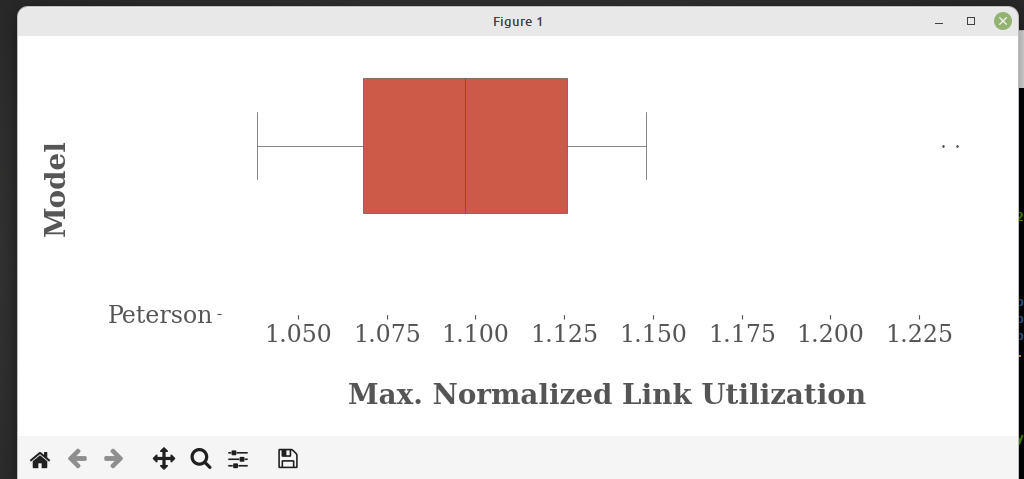
\includegraphics[width=\textwidth]{images/repr_daniel_10.png}
\end{center}
\end{frame}
\begin{frame}{Daniel}
\begin{center}
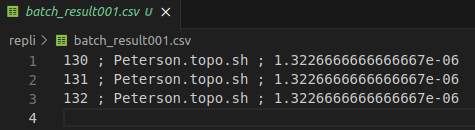
\includegraphics[width=\textwidth]{images/repr_daniel1.png}
\end{center}
\end{frame}
\begin{frame}{Zixiang Gu}
\begin{center}
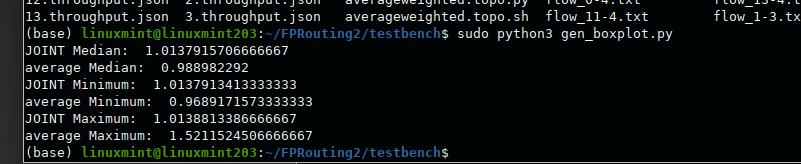
\includegraphics[width=\textwidth]{images/repr_zixiang1.png}
\end{center}
\end{frame}
\begin{frame}{Zixiang Gu}
\begin{center}s
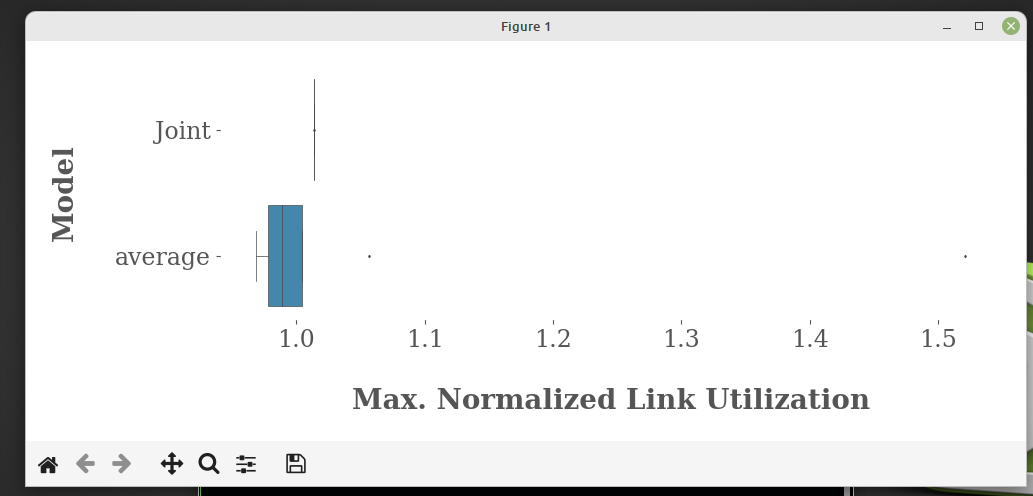
\includegraphics[width=\textwidth]{images/repr_zixiang_10.png}
\end{center}
\end{frame}

\begin{frame}[t,standout]
\Large
Fragen oder Anmerkungen?
\end{frame}
\end{document}

